%Papierformat
\documentclass[12pt,a4paper]{scrartcl}
%deutsche Silbentrennung
\usepackage[ngerman]{babel}
%Listen einrücken
\usepackage{enumitem}
%deutsche Umlaute
\usepackage[ansinew]{inputenc}
%Trennung von deutschen Umlauten
\usepackage[T1]{fontenc}
%für Zitate
\usepackage[numbers,square]{natbib}
%Grafikpaket laden
\usepackage{graphicx}
%Grafik Floating einschränken
\usepackage{placeins}
%Referenzierung mit Name
\usepackage{titleref}
%Unterschritszeilen
\usepackage{tabularx}
%Verlinkung
\usepackage{hyperref}
%urls sollen erkannt werden
\usepackage{url}

%\makeatletter
%\newcommand\footnoteref[1]{\protected@xdef\@thefnmark{\ref{#1}}\@footnotemark}
%\makeatother​

%Dokumentbeginn
\begin{document}

	%Festlegung des Zitatstyles - Harvardmethode: Abkuerzung Autor + Jahr
	\bibliographystyle{alphadin}

\begin{titlepage}
	%Eine mbox wird verwendet um Text zusammenzuhalten
	%vspace erzeugte die in Klammern angegebenen Zeilenabstände
	%baselineskip setzt zeilenabstand
   	\mbox{}\vspace{5\baselineskip}\\
   	%Schriftart und Größe als Attribut
   	\rmfamily\huge
   	%Mittige Textausrichtung (\centerline für eine Zeile)
   	\centering
   	%Das Argument erscheint in Kapitälchen (small capitals).
	\textsc{Security in iOS}
	%Umbruch bezogen auf die Höhe des Kleinbuchstaben x in diesem Element * Faktor
	\\[3ex]
   	Seminararbeit
   	\rmfamily\Large
   	\vspace{1\baselineskip}\\
   	%Externes einbinden einer Textdatei
   	\input{version.txt}\mbox{}
	\vspace{3\baselineskip}\\
	Hochschule f"ur angewandte Wissenschaften W"urzburg-Schweinfurt
   	\vspace{5\baselineskip}\\
   	\rmfamily\Large
   	David Artmann
   	\vspace{1\baselineskip}\\
   	%Heutiges Datum
   	\today
\end{titlepage}

	%Inhaltsverzeichnis
	\tableofcontents
	\newpage
	%Falls nötig...
	%Literaturliste im Inhaltsverzeichnis anzeigen
	%\addcontentsline{toc}{section}{Literatur}
	
	%Abbildungsverzeichnis
	\listoffigures
	
	%01.Vorwort
	\newpage
	\section{Vorwort}
	Die aus Cupertino in Kalifornien stammende US-Amerikanische Apple Corporation
	ist eine der gr��ten Firmen der Welt und hatte einen Umsatz von 182 Mrd.
	USD im Gesch�ftsjahr 2014. Sie ist ebenfalls der Erfinder des mobilen
	Betriebssystems iOS, welches auf den firmeneigenen Ger�ten iPad, iPad mini,
	iPhone, iPod touch und dem Apple TV ab der zweiten Generation zum Einsatz kommt.
	Der Kern des Betriebssystems basiert auf dem freien UNIX Betriebssystem Darwin,
	das auch als Vorlage f�r das Betriebssystem OS X genutzt wurde.\\
	Im Februar 2015 hatte iOS in den USA einen Marktanteil von 38,8\% und 17,4\%
	in Deutschland.
	\footnote{http://www.kantarworldpanel.com/global/smartphone-os-market-share/}
	Es existieren mehr als einhundert Millionen iPhones auf der ganzen Welt.\\
	Das Smartphone ob iOS, Android oder Windows Phone als Betriebsystem, ist in
	unserer heutigen Welt nicht mehr wegzudenken und mehrere Studien haben offen
	gelegt, dass das Smartphone den Computer bzw. Laptop - zumindest bei der
	Generation unter 18 Jahren - schl�gt.
	\footnote{http://www.bitkom.org/files/documents/BITKOM\_PK\_Kinder\_und\_Jugend\_3\_0.pdf}
	\footnote{http://www.mpfs.de/fileadmin/JIM-pdf13/JIMStudie2013.pdf}\\
	Welche Auswirkung h�tte es, wenn Sicherheitsl�cken auf diesen zu finden w�ren,
	oder schlimmer noch, diese v�llig ohne das Wissen des Nutzers ausgenutzt werden k�nnten?
	Mit dieser Arbeit m�chte ich besonders auf Sicherheitstechnische
	Problematiken dieses Betriebssystems eingehen und zeigen, dass ein Propriet�res
	Betriebssystem viele Vorteile hat, aber ebenso auch Nachteile besitzt die es nicht zu verachten gilt. 
	Ebenso werde ich versuchen mit praktischen Beispielen zu zeigen, dass iOS -
	obwohl propriet�r - dennoch angreifbar ist und L�cken aufweist.
	
	%02.Apple's law enforcement process guidelines
	\newpage
	\section{Apple's Law Enforcement Process Guidelines}
	Die Firma Apple schreibt auf ihrer Webseite:
	\begin{quote}
	Our commitment to customer privacy doesn't stop because of a government
	information request.
	\end{quote}
	Weiterhin wird beteuert: 
	\begin{quote}
	In addition, Apple has never worked with any government agency from any country to create a back 
	door in any of our products or services.
	\end{quote}
	Apple beteuert hier, seine Verpflichtung zur Einhaltung der Privatssphäre des
	Kunden auch nicht einzustellen, wenn die Regierung um Auskunft genau dieser
	Daten bittet.\\
	Zusätzlich wird versichert, dass Apple niemals mit Regierungsbehörden
	jedweder Lander gearbeitet hat, um Trojaner in eines ihrer Produkte oder
	Dienstleistungen einzubauen.\\\\
	Eine Einhaltung dieser Richtlinien ist von Kundenseite natürlich gewünscht.
	Ob Apple hier wirklich Wort hält, werde ich auf den kommenden Seiten genauer
	beleuchten.

	
	%03.Sicherheitsarchitektur iOS
	\newpage
	\section{Sicherheitsarchitektur iOS}
	\subsection{Secure boot chain}
	Apple hat eine Kette aneinander gereihter, vom Vorg�nger abh�ngiger Prozesse
	entwickelt, um den Startvorgang m�glichst abzusichern und eine Manipulation
	der Low-Level Software auszuschlie�en, da iOS nur auf Ger�ten startet, welche
	auf diesem Wege erfolgreich validiert wurden. Dieses "`secure boot chain"'
	genannte Verfahren sieht vor, nach dem Start eines iOS Ger�tes zuerst
	Code aus einem nur lesbaren Speicherbereich auszuf�hren. Dieser hardware of
	trust genannte unver�nderbare Code ist bei der Manufaktur der Chips eingebettet 
	worden und somit implizit vertraulich. Das Boot ROM enth�lt zus�tzlich Apple's 
	�ffentlichen Schl�ssel des Root Zertifikats, welcher sicher stellt, dass der 
	Low-Level-Bootloader von Apple signiert ist, bevor er ausgef�hrt wird. 
	
	%\begin{figure}[h]
		%\centering
 		%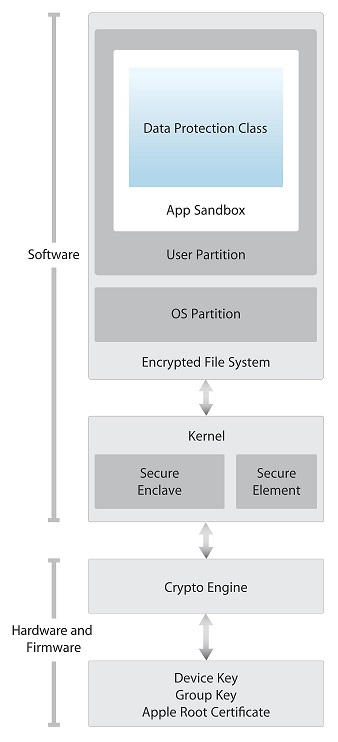
\includegraphics[width=0.3\linewidth]{ios/media/security-model.jpg}
        %\caption{Sicherheitsarchitektur Diagramm von iOS}
        %\label{fig:security-model}
    %\end{figure}\\
    %ref: Figure \ref{fig:security-model} shows the sec. arch.
    
    %\begin{wrapfigure}[Zeilen]{Position}[Ueberhang]{Breite}
	\begin{wrapfigure}[0]{r}[0.5cm]{6cm}
		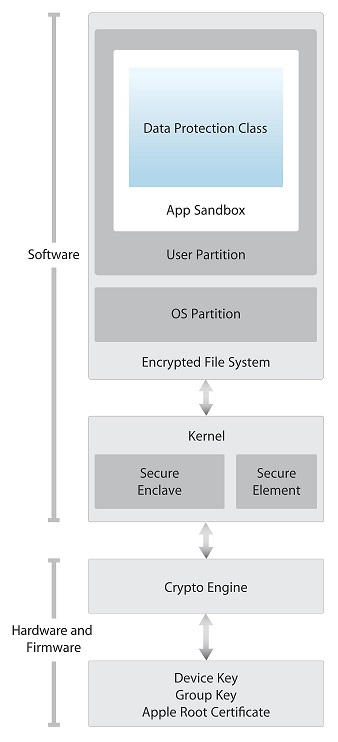
\includegraphics[width=\linewidth]{ios/media/security-model.jpg}
		\caption{Sicherheitsmodel von iOS}
		\label{fig:security-model}
	\end{wrapfigure}
	\subsection{iOS Sicherheitsmodel}
	Apple integrierte vier Schichten der Sicherheit in iOS.\\
	
	%04.Geheime Dienste
	\newpage
	\section{Geheime Dienste}
	Apple kann SMS, Fotos, Videos, Kontakte, Musik, Aufnahmen und Anruferhistorie
	aus passcode gesch�tzten Ger�ten auslesen. M�glich machen dies nicht
	dokumentierte Dienste, welche auf jedem Ger�t mit iOS installiert sind. In
	diesem Kapitel will ich auf diese Dienste eingehen und deren genauen
	Einsatzzweck erl�utern.
	\subsection{lockdownd - remote access}
	Der Dienst \textsl{lockdownd} erm�licht den Zugriff auf ein iOS Ger�t
	per TCP oder USB-Anschluss auf Port 62078.
	
	\newpage

\end{document}
